%%%%%%%%%%%%%%%%%%%%%%%%%%%%%%%%%%%%%%%%%%%%%%%%%%%%%%%%%%%%
\documentclass[xcolor=x11names,compress]{beamer}

\definecolor{CoolBlack}{rgb}{0.0, 0.18, 0.39}
\definecolor{byellow}{rgb}{0.55037, 0.38821, 0.06142}
%% General document %%%%%%%%%%%%%%%%%%%%%%%%%%%%%%%%%%
\usepackage{graphicx}
\usepackage{tikz}
\usepackage{Tabbing}
\usetikzlibrary{decorations.fractals}
%%%%%%%%%%%%%%%%%%%%%%%%%%%%%%%%%%%%%%%%%%%%%%%%%%%%%%

%% Beamer Layout %%%%%%%%%%%%%%%%%%%%%%%%%%%%%%%%%%
\useoutertheme[subsection=false,shadow]{miniframes}
\useinnertheme{default}
\usefonttheme{serif}
\usepackage{palatino}
\usepackage{tabu}

% addition of color
\usepackage{xcolor}
\definecolor{dgreen}{rgb}{0.,0.6,0.}
\definecolor{RawSienna}{cmyk}{0,0.72,1,0.45}

\setbeamerfont{title like}{shape=\scshape}
\setbeamerfont{frametitle}{shape=\scshape}

\setbeamercolor*{lower separation line head}{bg=CoolBlack} 
\setbeamercolor*{normal text}{fg=black,bg=white} 
\setbeamercolor*{alerted text}{fg=red} 
\setbeamercolor*{example text}{fg=black} 
\setbeamercolor*{structure}{fg=black} 
 
\setbeamercolor*{palette tertiary}{fg=black,bg=black!10} 
\setbeamercolor*{palette quaternary}{fg=black,bg=black!10} 

\renewcommand{\(}{\begin{columns}}
\renewcommand{\)}{\end{columns}}
\newcommand{\<}[1]{\begin{column}{#1}}
\renewcommand{\>}{\end{column}}

% adding slide numbers
\addtobeamertemplate{navigation symbols}{}{%
    \usebeamerfont{footline}%
    \usebeamercolor[fg]{footline}%
    \hspace{1em}%
    \insertframenumber/\inserttotalframenumber
}

% equation stuff
\newcommand{\Macro}{\ensuremath{\Sigma}}
\newcommand{\Sn}{\ensuremath{S_N} }
\newcommand{\vOmega}{\ensuremath{\hat{\Omega}}}
\usepackage{mathrsfs}
\usepackage[mathcal]{euscript}
\usepackage{amssymb}
\usepackage{amsthm}
\usepackage{epsfig}
\usepackage{amsmath}

\newcommand{\ve}[1]{\ensuremath{\mathbf{#1}}}
\newcommand{\micro}{\ensuremath{\sigma}}
\newcommand{\detR}{\ensuremath{\Sigma}}
%%%%%%%%%%%%%%%%%%%%%%%%%%%%%%%%%%%%%%%%%%%%%%%%%%

\begin{document}

%%%%%%%%%%%%%%%%%%%%%%%%%%%%%%%%%%%%%%%%%%%%%%%%%%%%%%
%%%%%%%%%%%%%%%%%%%%%%%%%%%%%%%%%%%%%%%%%%%%%%%%%%%%%%
\begin{frame}
\title{Research Plans}
\subtitle{Los Alamos National Laboratory}
\author{
        \includegraphics[height=2cm]{../bk}\\R.\ N.\ Slaybaugh, \\ Univ. of Cal.\ Berkeley}

\date{4 August 2014}
\titlepage
\end{frame}

% --------------------------------------------------------------
\begin{frame}[fragile]{Outline}
  \frametitle{Outline}
  \begin{itemize}
	\item MC importances for problems with strong anisotropies
	\begin{itemize}
	  \item Using the angular flux
	  \item LDO equations
	\end{itemize}
	\item Other potential projects
  \end{itemize}

\end{frame}


% --------------------------------------------------------------
% --------------------------------------------------------------
\section{\scshape Strong Anisotropies}
\begin{frame}[fragile]
  \frametitle{Anisotropy: a computational challenge}

	\begin{columns}
  	\begin{column}{0.5\textwidth}
	\begin{itemize}
	\item Many important nuclear applications have strong anisotropies
	 \begin{itemize}
	 \item Used fuel casks
	 \item Reprocessing facilities
	 \item Reactor facilities
	 \item Active interrogation 
	 \end{itemize}
	\item These are difficult to capture with current tools:
	 \begin{itemize}
	 \item Ray effects with deterministic
	 \item Too slow with analog MC
	 \item Insufficient acceleration of MC with hybrid
	 \end{itemize}
	\end{itemize}
  	\end{column}
 	%
 	\begin{column}{0.5\textwidth}
 	 \begin{center}
 	 \begin{figure}
 	 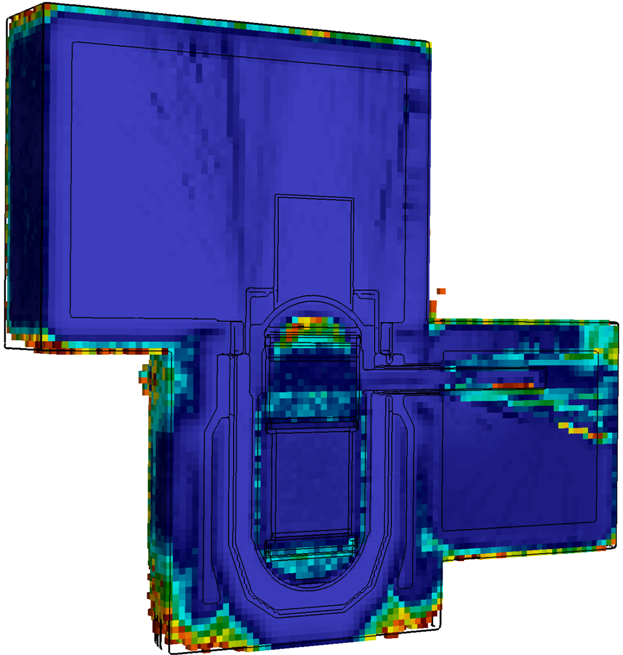
\includegraphics[height=2in,clip]{../figs/pwr}  
 	 \caption{PWR, 1 CPU-month, FW-CADIS  for mesh-tally (500K cells)}
 	 \end{figure}
 	 \end{center}

  	\end{column}
	\end{columns}

\end{frame}

% --------------------------------------------------------------
\begin{frame}[fragile]
  \frametitle{Many Attempts at Resolution; Mixed Success}

	\begin{itemize}
	\item Automatic WW generator
	\item AVATAR
	\item LIFT
	\item Cooper and Larsen's global weight windows
	\item CADIS/FW-CADIS
	\item Resonance Factor method
	\end{itemize}

\end{frame}

% --------------------------------------------------------------
\begin{frame}[fragile]
  \frametitle{Current global hybrid methods are insufficient}

	\begin{itemize}
	\item MC VR parameters created from adjoint deterministic flux that is a function of \emph{space and energy only}
	\item Angular dependence of the importance function is not retained, otherwise the map would be
	  \begin{itemize}
	  \item very large (tens or hundreds of GB)
	  \item more costly and complex to use in MC simulation
      \end{itemize}	   
	\item Drawback: within a given space/energy cell, the map provides the \emph{average} importance of a particle moving in \emph{any direction} through the cell -- excluding information about how particles move \underline{toward} the objective
	\end{itemize}

\end{frame}

% --------------------------------------------------------------
\begin{frame}[fragile]
  \frametitle{Current hybrid methods are insufficient}

	\begin{columns}
  	\begin{column}{0.5\textwidth}
 	 \begin{center}
 	 \begin{figure}
 	 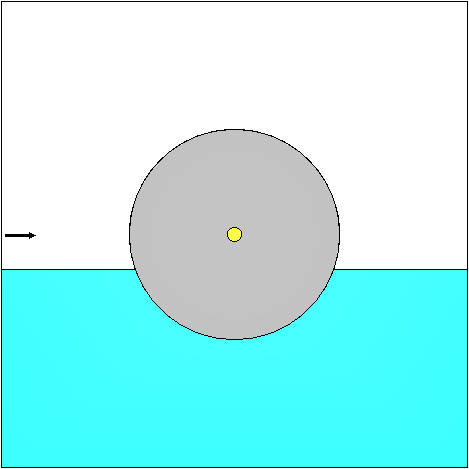
\includegraphics[height=2in,clip]{../figs/boat-interrogation}  
 	 \caption{Spherical boat model with source on left and fissionable material at center}
 	 \end{figure}
 	 \end{center}
  	\end{column}
 	%
 	\begin{column}{0.5\textwidth}
 	 \begin{center}
 	 \begin{figure}
 	 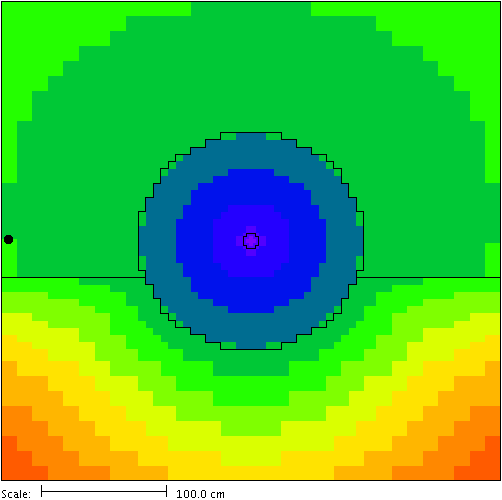
\includegraphics[height=2in,clip]{../figs/boat-map}  
 	 \caption{Target CADIS weight window values for 14.1 MeV neutrons}
 	 \end{figure}
 	 \end{center}
  	\end{column}
	\end{columns}

\end{frame}

% --------------------------------------------------------------
\begin{frame}[fragile]
  \frametitle{Better hybrid methods are needed}

	\begin{itemize}
	\item We can use angular information to improve performance
		\begin{equation}
		\phi^{\dagger}(\ve{r},E) = \frac{\int \psi(\vOmega, \ve{r},E) \psi^{\dagger}(\vOmega, \ve{r},E) d\vOmega}{\int \psi(\vOmega, \ve{r},E)  d\vOmega}
		\end{equation}

	\item The space- and energy-dependent importance map will be normalized and source biasing parameters will be generated in a manner similar to the current implementation of hybrid methods
	\item Immediately useful; widely applicable
	\end{itemize}

\end{frame}


% --------------------------------------------------------------
\begin{frame}[fragile]
  \frametitle{Lagrange Discrete Ordinate Equations}

	\begin{itemize}
	\item Re-derivation of $S_N$ with an interpolatory quadrature framework
	\item Allows evaluation at directions not on quadrature set
	\item No need to store spherical harmonic moments
	\item May be useful for more accurately capturing strong anisotropies
	\end{itemize}
	
	Use as standalone or in FW-CADIS?

\end{frame}

% --------------------------------------------------------------
% --------------------------------------------------------------
\section{\scshape Other Projects}
\begin{frame}[fragile]
  \frametitle{Other (potential) projects}

  	\begin{itemize}
  	\item Continuing development of MC on GPU
  	\item Contributing methods to PyNE; investigating a long term research relationship 
	\item 3D shielding optimization: applicable to SMRs 
	%\item Parallelization of open source deterministic code, Detran 
	\item Investigating use of hybrid methods for interrogation of SNM with neutron time-correlations 
	%\item Using SP$_N$ in multigrid preconditioner in Denovo 
	\end{itemize}
	
\end{frame}



\end{document}